\section{Durchführung}
\label{sec:Durchführung}

Zunächst wird der Versuchsaufbau und die Durchführung des jeweils zu untersuchenden Objekts beschrieben.
Der Aufbau besteht dabei aus einem Ultraschallechoskop, Ultraschallsonden sowie einem Rechner für die Datenanalyse mit dem Programm \enquote{EchoView}.
Für die jeweilige Messmethode werden dabei eine oder zwei gleiche Sonden eingesetzt. 
Als Kontaktmittel wird zunächst für die Acrylobjekte bidestilliertes Wasser verwendet.
Die Ergebnisse können in sogenannten A-Scan's, B-Scan's oder TM-Scan's gespeichert und dargestellt werden.

Am Anfang der Durchführung wird mithilfe einer Acrylplatte die Schallgeschwindigkeit mittels Impuls-Echo-Verfahren bestimmt.
Diese wird nach Abgleich mit der Theorie dem Programm übergeben, um die Messtiefe der Sonde in $\unit{\milli\meter}$ angeben zu können.


\subsection{Bestimmung der Schallgeschwindigkeit mit dem Impuls-Echo-Verfahren} \label{sec:schallecho}

Hierfür werden Acrylzylinder verschiedener Längen zunächst mit eine Schieblehre vermessen. 
Anschließend wird ein senkrecht stehender Zylinder mit einer Sonde von oben gekoppelt und mit einem A-Scan die Laufzeit bestimmt.
Dies wird für sieben verschiedene Längenanordnungen wiederholt und bei einem schwachen Signal eine 
laufzeit- bzw. tiefenabhängige Verstärkung (\enquote{Time Gain Control}) zugeführt, welches am Echoskop reguliert werden.


\subsection{Bestimmung der Schallgeschwindigkeit mit dem Durchschallungs-Verfahren}

Zur Durchschallung eines Zylinders wird dieser waagerecht zwischen zwei Sonden mit Ultraschallgel gekoppelt und für alle Zylinder wiederholt.


\subsection{Bestimmung der Dämpfung mit dem Impuls-Echo-Verfahren}

Die Messung für die Bestimmung der Dämpfung erfolgt hierbei analog zu \autoref{sec:schallecho}, 
nur das dabei zur Messung der Amplituden darauf zu achten ist, dass TGC ausgestellt wird und die Messung nicht verfälscht.


\subsection{Vermessung des Augenmodells}

\begin{figure}
    \centering
    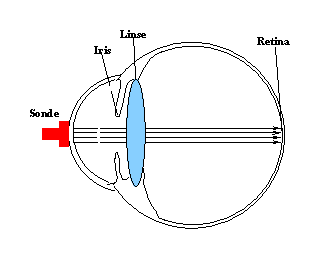
\includegraphics[width=0.4\linewidth]{pictures/auge.pdf}
    \caption{Bestandteile des Augenmodells (Maßstab 1:3). \cite{us1}}
    \label{fig:augenmodell}
\end{figure}

Zur Abmessung des Augenmodells in \autoref{fig:augenmodell} wird mithilfe des Impuls-Echo-Verfahrens die Laufzeit von Augeneingang zur Retina bestimmt.
Dafür wird mit Koppelgel mit leichtem Druck auf der Hornhaut die Sonde platziert, bis ein Echo an der Rückwand der Retina zu sehen ist.


\subsection{Vorbereitungsaufgabe}

Als Vorbereitungsaufgabe soll zunächst die Schallgeschwindigkeit c verschiedener Materialien nach \cite{schallgeschw}, \cite{schallgeschw2} und \cite{schallgeschw3} angegeben werden.
Die akustische Feldimpedanz lässt sich mithilfe der Gleichung
\begin{equation*}
    Z = \rho \cdot c
\end{equation*}
berechnen, wobei $\rho$ die Stoffdichte ist. Mit den Dichten der Stoffe nach \cite{akimpedanz} folgt somit für die Impedanzen:
\begin{align*}
    c_\text{Luft}           =  \qty{331}{\meter\per\second} \quad &\implies \quad Z_\text{Luft}           = \qty{0.43e5}{\kilo\gram\per\meter\squared\per\second} \\
    c_\text{Wasser}         = \qty{1492}{\meter\per\second} \quad &\implies \quad Z_\text{Wasser}         = \qty{1.49e6}{\kilo\gram\per\meter\squared\per\second} \\
    c_\text{Blut}           = \qty{1570}{\meter\per\second} \quad &\implies \quad Z_\text{Blut}           = \qty{1.64e6}{\kilo\gram\per\meter\squared\per\second} \\
    c_\text{Knochen}        = \qty{3500}{\meter\per\second} \quad &\implies \quad Z_\text{Knochen}        = \qty{6.12e6}{\kilo\gram\per\meter\squared\per\second} \\
    c_\text{Acryl}          = \qty{2730}{\meter\per\second} \quad &\implies \quad Z_\text{Acryl}          = \qty{3.22e6}{\kilo\gram\per\meter\squared\per\second} 
\end{align*}
Schließlich soll noch die Wellenlänge $\lambda$ und die Periode T einer $\qty{2}{MHz}$ Schwingung in Acryl angegeben werden:
\begin{align*}
    T = \frac{1}{\qty{2}{MHz}} = \qty{0.5e{-6}}{\second} \qquad \qquad \lambda = \frac{c}{f} = \qty{1.365e{-3}}{m}
\end{align*}